\documentclass{standalone}
\usepackage{tikz}
\usepackage{ctex,siunitx}
\setCJKmainfont{Noto Serif CJK SC}
\usepackage{tkz-euclide}
\usepackage{amsmath}
\usetikzlibrary{patterns, calc,3d}
\usetikzlibrary {decorations.pathmorphing,decorations.pathreplacing,decorations.shapes}
\tikzset{label style/.append style={font=\small}}
\begin{document}
\small
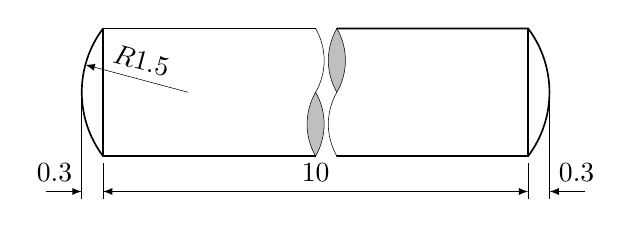
\begin{tikzpicture}[>=latex,scale=0.9]
  \tkzDefPoints{0/0/A,0/1.8/B,1.2/0.9/O,3/0/M,3/1.8/N,3.3/0/P,3.3/1.8/P'}
  \tkzDefPointsBy[reflection=over M--N](A,O,B){A',O',B'}
  \tkzDrawArc[semithick](O',A')(B')
  \tkzDrawArc[semithick](O,B)(A)
  \tkzDrawSegments[semithick](M,A A,B A',B' B',P' A',P B,N)
  \fill[lightgray](M)arc(-30:30:0.9)arc(150:210:0.9);
  \fill[lightgray](P')arc(150:210:0.9)arc(-30:30:0.9);
  \draw[very thin](N)arc(30:-30:0.9)arc(150:210:0.9)arc(-30:30:0.9);
  \draw[very thin](P)arc(-150:-210:0.9)arc(-30:30:0.9)arc(150:210:0.9);
  \draw[very thin](0,-0.1)--(0,-0.6)(6,-0.1)--(6,-0.6)(-0.3,0.8)--(-0.3,-0.6)(6.3,0.8)--(6.3,-0.6);
  \draw[very thin,<->](0,-0.5)--(6,-0.5)node[midway,above]{10};
  \draw[very thin,->](-0.8,-0.5)--(-0.3,-0.5)node[above left]{0.3};
  \draw[very thin,->](6.8,-0.5)--(6.3,-0.5)node[above right]{0.3};
  \draw[very thin,->](O)--++(165:1.5)node[midway,sloped,above]{$R1.5$};
\end{tikzpicture}
\end{document}